\documentclass{article}
\usepackage{graphicx} % Required for inserting images
\usepackage{listings} % useful for putting code in

\title{ML Course Chapter 6}
\author{Samuel Wang}
\date{August 2025}

\begin{document}

\maketitle

\section{Lab}

\subsection{Question 1}

\subsubsection{1.1}

\paragraph{A: } Since this network only has 1 layer, the separator produced is linear.

\paragraph{B: } With a step size of 0.1 and 1,000 iterations, I essentially always end up with an accuracy of $1$.

\subsubsection{1.2}

\paragraph{A: } 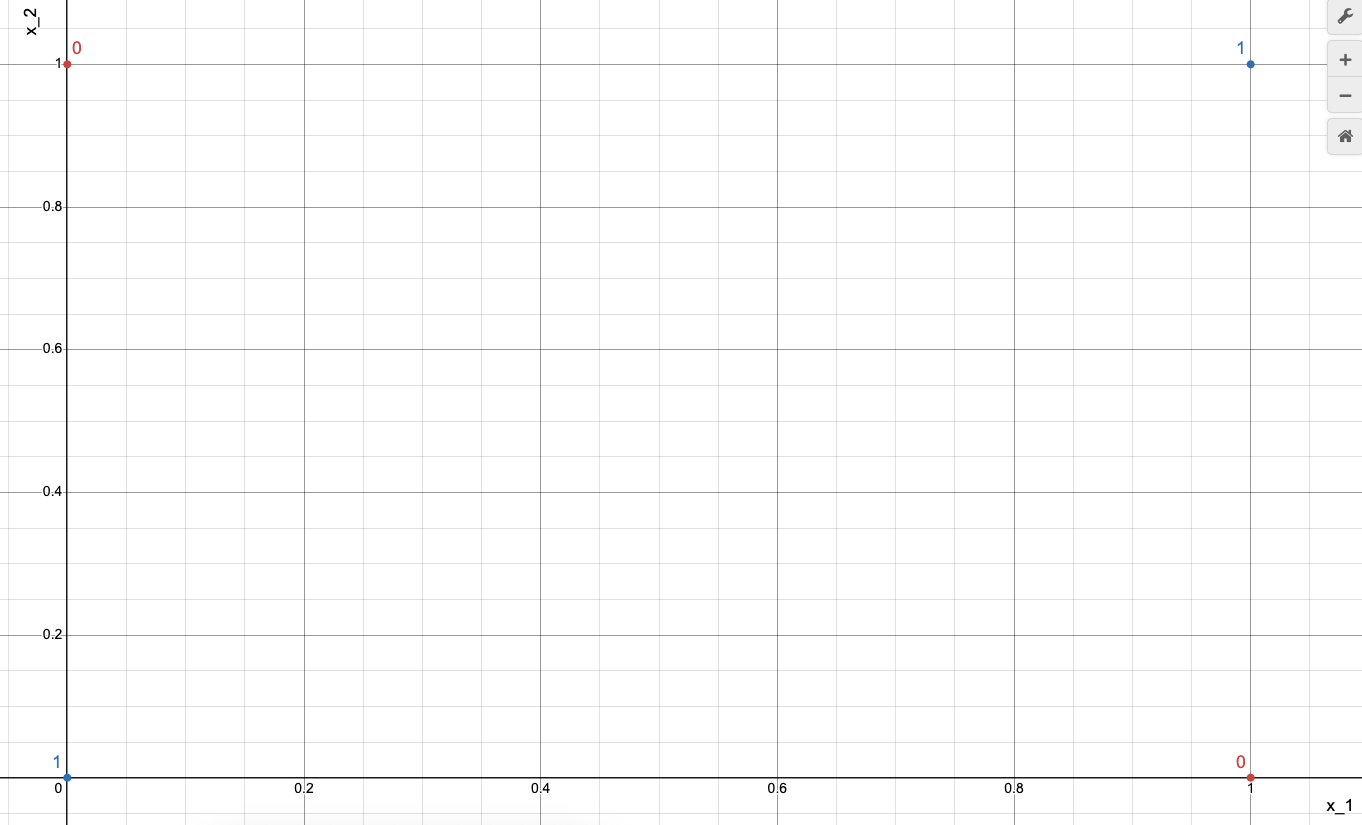
\includegraphics[width=5cm, height=4cm]{Week 6 graph.png}

\paragraph{B: } With only $1$ hidden unit, this problem is impossible, as when we are reduced to a single hidden unit, we will have reduced the problem to a linear one, which in the case of XOR cannot solve the problem with 100\% accuracy. With 2 hidden units, the algorithm is likely to be non-linear, so this should theoretically work.

\paragraph{C: } After running, it seems that $3$ hidden units were actually required to consistently classify, as $2$ units led to another linear classifier. My best guess as to why this happens is that with less than $3$ hidden units, mathematically working through the algorithm somehow gives us an overall linear separator.

\subsubsection{1.3}

\paragraph{A: } I was able to get 95\% accuracy with 4 hidden units, 1000 iterations, and a step size of 0.05. I don't think 100\% accuracy is practical within a reasonable amount of time.

\paragraph{B: } For this data set, I believe a "perfect" separator on the training set is inadvisable, since this set contains a single positive data point very deep into what would reasonably be considered parts that negative points would be contained in. So, a "perfect" separator would not only take a while to train, but would also be overfitted, and likely do worse on test cases than our 95\% accurate classifier.

\subsection{Question 2}

\paragraph{A: } For the input, for the sake of optimization, I would vectorize the words in the title, and add the vectors together to form the vector of the title as a whole. The output would be a single value, that being the predicted change in the stock market, in points. The loss function would simply be the squared difference between the predicted change for a particular headline and the actual change that day. In terms of the activation function, I think linear is a good choice, since we are trying to predict a single value which can vary between several different values.

\paragraph{B: } For the input, I would train a separate encoder and decoder to compress the image into a 1-dimensional vector, and decompress the vector back into a decent reconstruction of the original image. In terms of the output layer, I'd simply have the output be a single value, that being the probability. For the activation function, sigmoid makes the most sense, as it allows us to convert any real number efficiently into a probability. The loss function would likely be NLL, as we are predicting a probability, and thus it makes the most sense to calculate loss by the probability we predict incorrectly.

\paragraph{C: } The input would be vectorized the same way as in 2A. As for the output, it would be a vector, consisting of the confidence the algorithm thinks it belongs in each folder. For the activation function, softmax makes most sense, as we are predicting between multiple different disjoint labels, and need a way to regularize the real-valued outputs we get. For loss, quadratic makes most sense, since we are looking for the difference between 2 vectors, one being our output and the other being the expected one-hot encoded vector.

\paragraph{D: } Input would be vectorized the same way as in 2A and 2C. For the output, it would have to be a vector, where each output is the probability the algorithm thinks the topic has of occurring. The activation would be vector sigmoid, since we want to convert a real-valued vector to a vector of probabilities, but also do not want to limit the sum of the probabilities to 1, as this document may contain multiple topics. For the loss, quadratic makes the most sense for the same reason as 2C.

\end{document}